\chapter{Detección de nadadores mediante técnicas clásicas } \label{cap:capitulo3}

En este capítulo abordaremos la detección del nadador en la piscina mediante técnicas clásicas del procesamiento de imágenes, separando el problema en tres apartados. En primer lugar, trataremos la importancia de una correcta selección del espacio de color sobre el que trabajar. Como segundo paso abordaremos la sustracción de fondos para distinguir los elementos estáticos de los dinámicos. Por último, obtendremos las bounding boxes que contienen al nadador. La sección concluye con una evaluación experimental que compara las distintas aproximaciones.

\section{Espacios de color}

Una de las primeras decisiones que debemos tomar cuando tenemos que procesar una imagen es el espacio de color en el que vamos a representar la información.

Las fotografía o vídeos que visualizamos diariamente, mediante la multitud de pantallas que nos rodean continuamente, suelen utilizar el espacio de color RGB, pero este no es el único modelo de color en que podemos representar nuestras imágenes; existen otras alternativas como HSV e YCbCr. A continuación, vamos a comentar las características de cada uno de estos tres espacios de color y su posible utilidad en nuestro problema. La elección de estos tres espacios de color concretos, RGB, HSV e YCbCr, viene motivada por su uso en publicaciones anteriores, tales como \cite{swimmerarti} y \cite{swimmerartii}. Nótese que este trabajo no pretende ser una revisión exhaustiva de los modelos de color y tan solo se recogen los que van a ser utilizados.

\subsection{RGB}

El espacio de color RGB es un espacio de color aditivo, en el que cada posible color se representa mediante la mezcla por adición de otros colores base \cite{abitofallcolorspaces}. En concreto, se utilizan los tres colores primarios aditivos; rojo (R), verde (G) y azul (B). Sin embargo, este modelo de color no define por sí mismo qué son los colores rojo, verde y azul, por lo que su representación puede diferir en función del dispositivo y del tipo de elemento físico que utilice cada uno de ellos para producir la luz, y por tanto, cada uno de los colores.

El esquema de representación del color RGB fue propuesto por primera vez en 1809 por el físico y oftalmólogo inglés Thomas Young. Según su trabajo en \cite{rgbtrivision}, la visión humana es tri-cromática dado que en la retina  disponemos de tres sensores para la percepción del color – los conos L, S y M -, siendo cada uno de ellos especialmente sensible a longitudes de onda diferentes, correspondientes a los colores primarios aditivos anteriormente mencionados. Una consecuencia de este hecho es que las representaciones de color sean también tri-cromáticas. Cuando los colores primarios se mezclan entre sí por parejas en la misma proporción aparecen los colores secundarios, el magenta, azul cian y amarillo. Para obtener el blanco mezclamos los tres colores primarios, mientras que para obtener el negro simplemente debemos no utilizar color alguno. Este sistema permite la definición y visualización de un gran número de colores, proporcional al número de bits que utilicemos para representar la cantidad de cada color primario. Por ejemplo, si utilizamos 8 bits para cada color primario podremos representar 16.777.216 colores.

Para representar el conjunto de colores RGB se suele emplear cubos como los que se muestran en la figura \ref{fig:cubosRGB}.

\begin{figure}[h!]
    \centering
    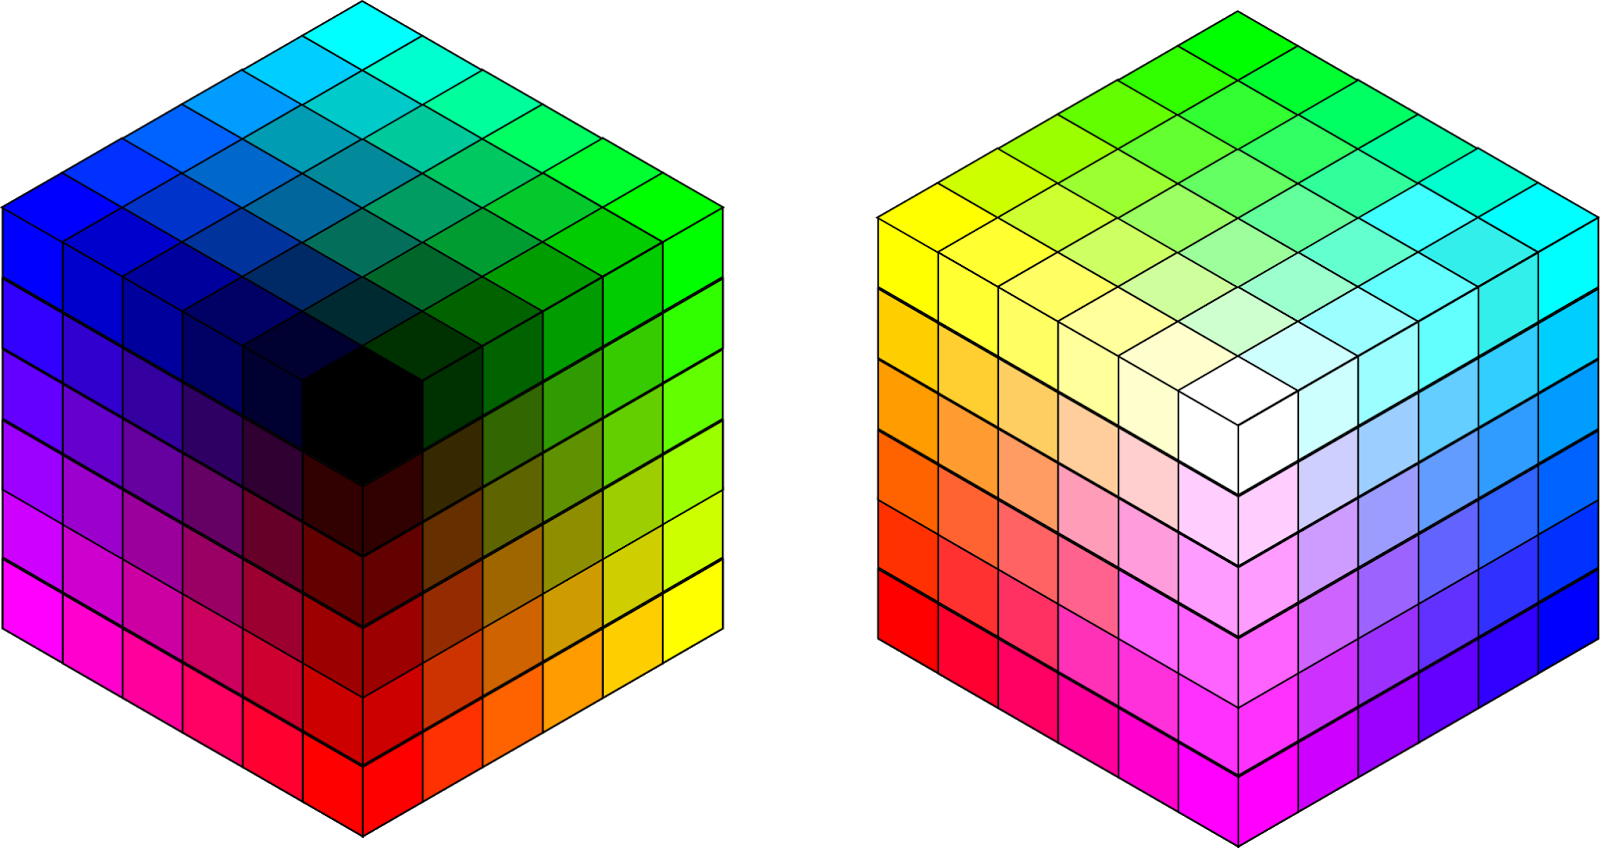
\includegraphics[width=0.7\textwidth,height=0.7\textheight,keepaspectratio]{imagenes/parte_BS/cubos_rgb.png}    
    \caption{Representación del espacio de color RGB.}
    \label{fig:cubosRGB}
\end{figure}

RGB es un modelo de color, es decir, es una representación matemática que describe cómo se combinan los colores primarios. Sin embargo, hay multitud de espacios de color RGB distintos, con diferentes parámetros, que han sido creados con el paso del tiempo ante la necesidad de los consumidores, intereses profesionales o avances tecnológicos. También existen multitud estándares que determinan que parámetros deben usarse en qué situaciones \cite{rgbtrivision}. Podemos mencionar los espacios \textit{sRGB}, \textit{AdobeRGB}, \textit{CIE 1931 RGB}, \textit{NTSC} y \textit{DCI-P3}; y los estándares \textit{SMPTE-C}, \textit{ITU-R BT.601} e \textit{ITU-R BT.709-3}.

\subsection{HSV}

El modelo de color HSV, creado por Alvy Ray Smith en 1978 \cite{abitofallcolorspaces}, tiene como principal objetivo representar con mayor exactitud la forma en la que la visión humana percibe los atributos que componen cada color.

Para representar los colores este modelo utiliza tres componentes, llamadas tono (hue), saturación (saturation) y valor (value). Pasemos a describir cada componente \cite{libroTID}.
\begin{itemize}
    \item El tono representa el atributo de una sensación visual según la cual un área parece similar al color rojo, amarillo, verde, azul o a una combinación de dos de los colores anteriores en respuesta a la longitud de onda de la luz captada. La gama cromática se suele representar en una rueda o cono circulares, como se puede apreciar en la figura \ref{fig:conoHSV}, de manera que se indica el color mediante un ángulo entre 0 y 360 grados. En particular, un ángulo de 0º corresponde al rojo, uno de 120º corresponde al verde y uno de 240º corresponde al azul.
    \item La saturación indica la cantidad de color que tenemos en un área en proporción a su brillo, es decir, su pureza; o dicho de otro modo, la cantidad de blanco que se encuentra embebida en un color concreto. Este valor se representa como un número entre 0 y 1, o un porcentaje entre 0 y 100.
    \item El valor representa el atributo de una sensación visual según el cual un área parece emitir más o menos luz. Una vez más, el valor se representa mediante un porcentaje entre 0 y 100 o un número entre 0 y 1.
\end{itemize}

\begin{figure}[h!]
    \centering
    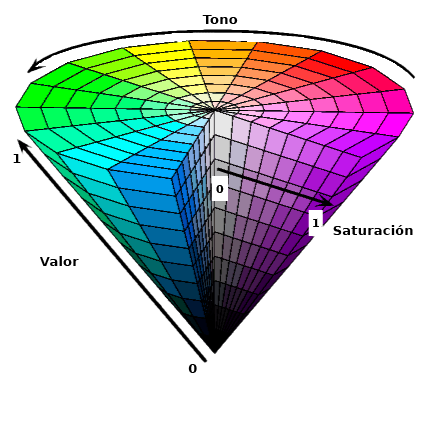
\includegraphics[width=0.5\textwidth,height=0.5\textheight,keepaspectratio]{imagenes/parte_BS/cono_hsv.png}    
    \caption{Representación del espacio de color HSV.}
    \label{fig:conoHSV}
\end{figure}

Existen otros modelos (HSI y HSL) que comparten los conceptos de tono y saturación y se consideran de la misma familia. No ocurre lo mismo con el concepto de valor, que se sustituye por intensidad y luminancia respectivamente. HSI y HSL no se utilizan en este trabajo, pero el lector interesado puede consultar las diferencias en \cite{abitofallcolorspaces}.

\subsection{YCbCr}

El modelo de color YCbCr es ampliamente usado para la representación de vídeo digital – especialmente en televisión - dado que forma parte de la recomendación \textit{ITU-R BT.601} de la \textit{ITU (International Telecommunication Union)} que se sigue en la Unión Europea \cite{abitofallcolorspaces}. 

Este modelo de color utiliza tres componentes, una de luminancia y dos de crominancia, para representar los colores.

\begin{itemize}
    \item Y: componente de luminancia que representa la intensidad del brillo del color. Por sí misma permite representar imágenes en blanco y negro.
    \item Cb: componente diferencial de crominancia azul, es decir, la diferencia entre luminancia y el valor azul.
    \item Cr: componente diferencial de crominancia roja. Representa la diferencia entre luminancia y el valor rojo. 
\end{itemize}

Según \cite{featureextraction}, el estándar obliga, para representaciones de 8 bits, a que el valor de la componente de luminancia esté comprendido entre los valores 16 y 235, mientras que los valores de las componentes de crominancia deben ser inferiores a 240. Esto se hace para que la conversión a RGB no produzca colores que dicho espacio de color no sea capaz de representar.

En la figura \ref{fig:planosycbcr} podemos observar la representación del plano Cb/Cr para diferentes valores de luminancia.

\begin{figure}[h!]
    \centering
    \begin{tabular}{ccc}
          
\includegraphics[width=0.28\textwidth,height=0.28\textheight,keepaspectratio]{imagenes/parte_BS/YCbCr_Y0.png} & 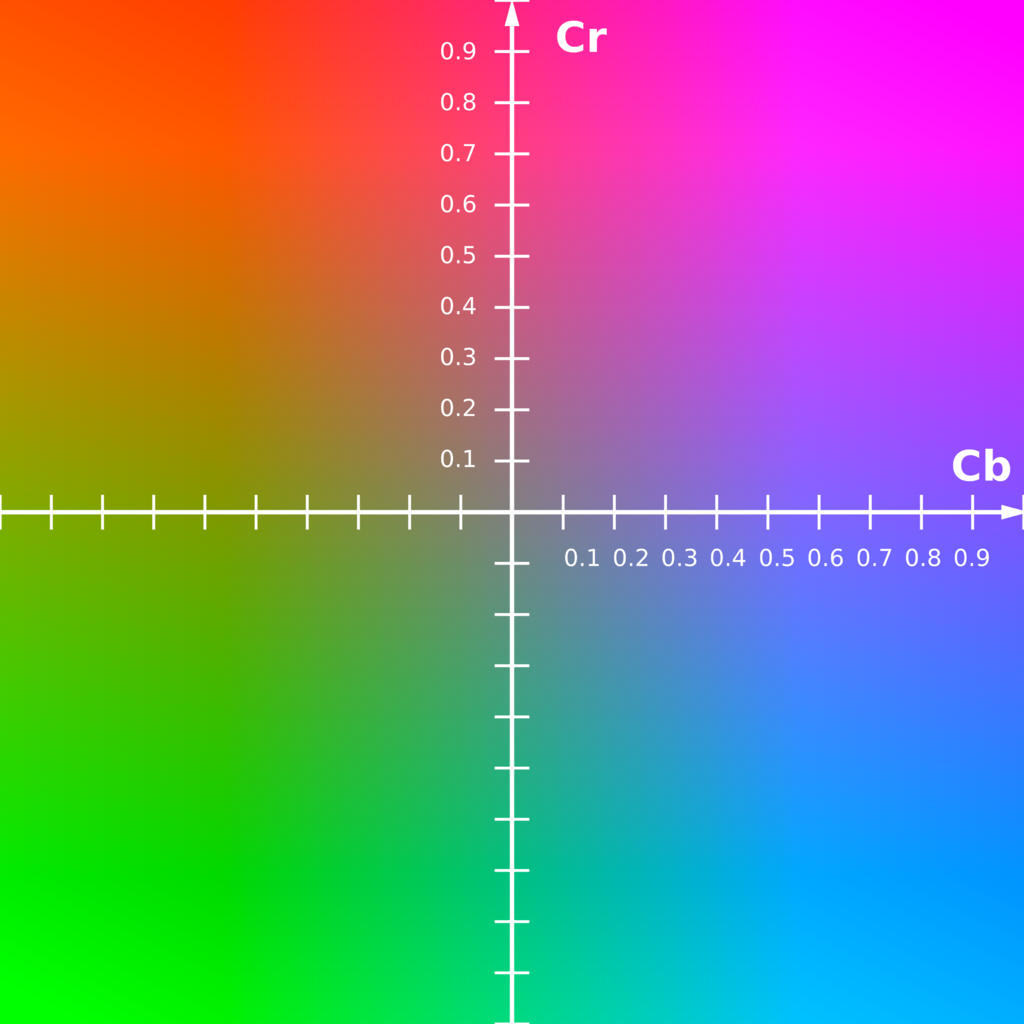
\includegraphics[width=0.28\textwidth,height=0.28\textheight,keepaspectratio]{imagenes/parte_BS/YCbCr_Y50.png} &
          
\includegraphics[width=0.28\textwidth,height=0.28\textheight,keepaspectratio]{imagenes/parte_BS/YCbCr_Y100.png} \\
          a) Y=0 & b) Y=0.5 & c) Y=1\\
     \end{tabular}
     \caption{Planos Cb/Cr para diferentes luminancias.}
     \label{fig:planosycbcr}
\end{figure}

En ocasiones, YCbCr e Y’CbCr se usan indistintamente, a pesar de ser modelos de color distintos \cite{moredigitalvideo}. En la versión con apóstrofo se utiliza corrección gamma, por lo que la componente de luminancia tendrá un valor en el rango [0, 1], mientras que las componentes de crominancia tendrán un valor en el intervalo [-0.5, 0.5]. A la hora de elegir un paquete software para tratamiento de imágenes deberemos tener en cuenta si permite el uso de ambos espacios de color, o en su defecto, cual de los dos se utiliza concretamente. Adicionalmente, tenemos que tener en cuenta que se suelen realizar conversiones de tal manera que los valores oscilen en el rango [0, 255].

En el modelo de color YCbCr se suele utilizar submuestreo de las componentes de crominancia \cite{submuestreocroma}. Codificando menos información de color que de luminancia, las imágenes ocupan menos espacio y su transmisión requiere un menor ancho de banda. Esta codificación no resulta en una degradación apreciable de la calidad de la imagen dado que el ojo humano es más sensible a la luminancia que al color \cite{submuestreocroma}.

Los diferentes formatos de submuestreo cromático se suelen representar mediante la notación X:Y:Z, donde X representa el tamaño de una región horizontal de muestreo - habitualmente de 4 píxeles - Y nos dice cuantas muestras para cada banda de crominancia se toman en una fila de largo X píxeles, y Z nos indica cuantos cambios en las muestras de crominancia hay entre la primera y segunda fila de X píxeles \cite{submuestreocroma}.

Los tres esquemas más utilizados son los siguientes:
\begin{itemize}
    \item 4:4:4. Para cada píxel muestreamos cada una de las componentes, por lo que no se produce compresión ni reducción de la calidad.
    \item 4:2:2. Para cada píxel muestreamos la componente de luminancia, pero las componentes de crominancia se muestrean para uno de cada dos píxeles horizontales.
    \item 4:2:0. Para cada píxel se muestrea la componente de luminancia, pero las componentes de crominancia se muestrean en un único píxel de una región 2x2 píxeles. 
\end{itemize}
Para un mejor entendimiento, en la figura \ref{fig:subsamplingycbcr} se puede apreciar el efecto de aplicar cada una de estas técnicas de submuestreo cromático. Cuanto menor sea el número de componentes de crominancia muestreadas, más similares serán los colores de una región 2x2 entre sí, a la vez que más diferentes de los colores originales.

\begin{figure}[h!]
    \centering
    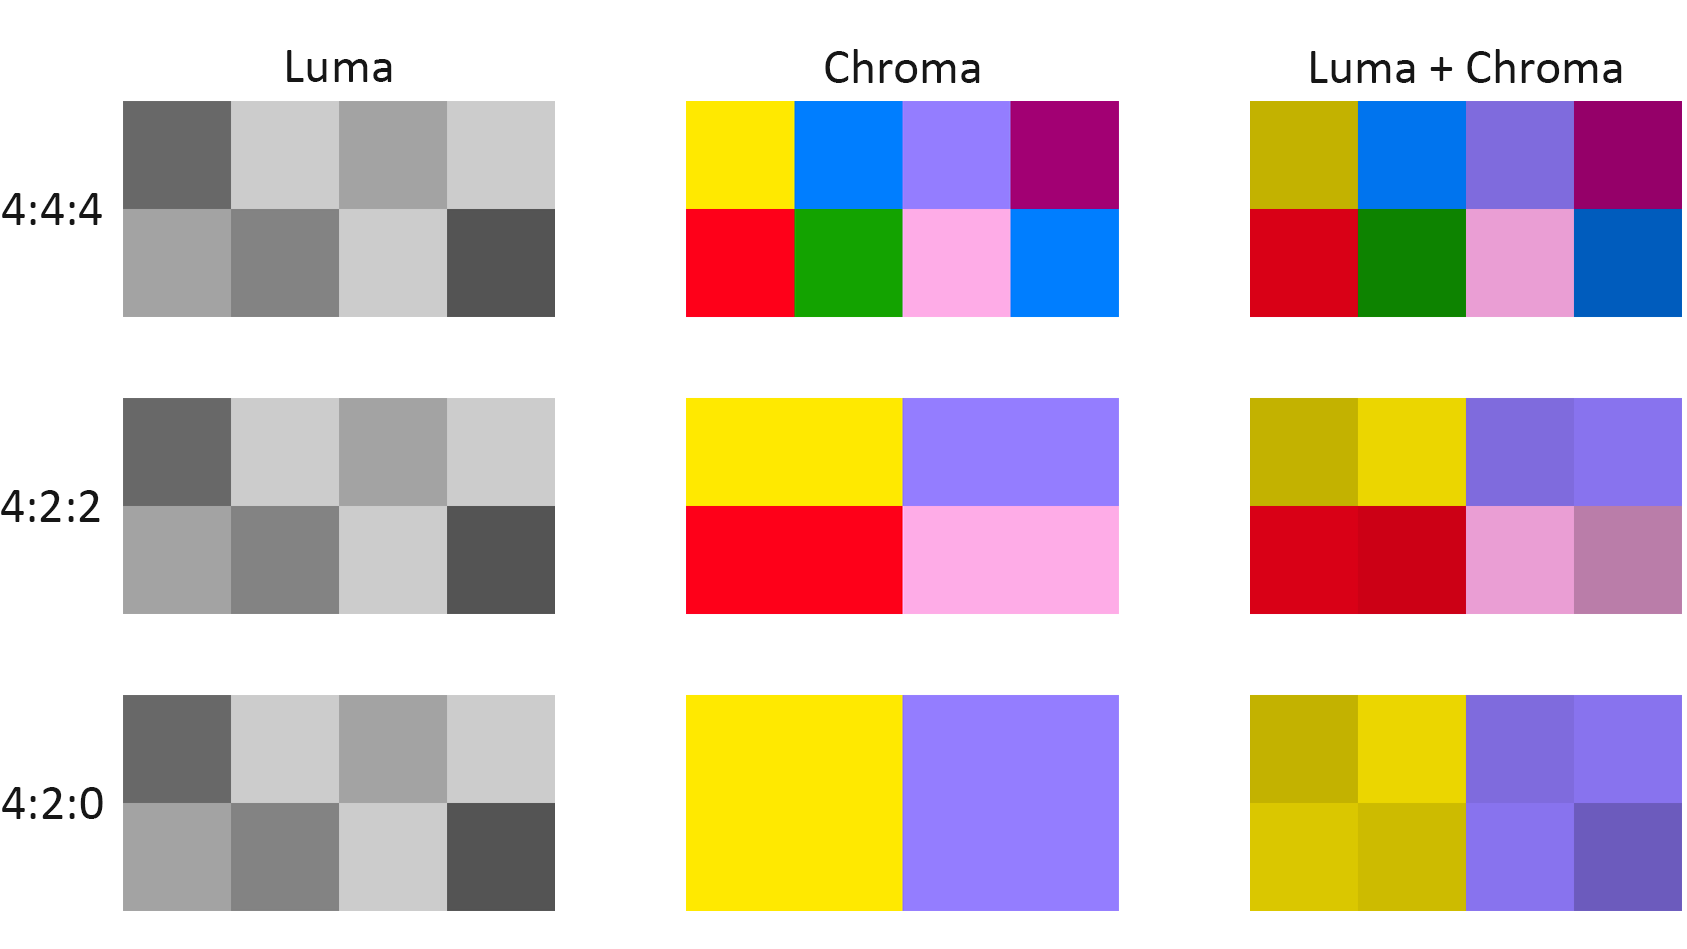
\includegraphics[width=0.65\textwidth,height=0.65\textheight,keepaspectratio]{imagenes/parte_BS/subsamplingycbcr.png}    
    \caption{Esquemas de submuestreo cromático.}
    \label{fig:subsamplingycbcr}
\end{figure}

\subsection{Elección del espacio de trabajo para la detección de nadadores y su justificación} \label{sub:elegirespaciocolor}

Una vez hemos comentado las características de los principales espacios de color, pasamos a analizar la posible utilidad de cada uno de ellos en nuestro problema concreto, la detección de nadadores. Realizamos este análisis dado que trabajos anteriores, como \cite{hsvforswimmerdetection}, \cite{swimmerartii}, \cite{footbalhsv} y \cite{swimmerdetectorii}, sugieren que la correcta elección del espacio de color influye significativamente en el rendimiento de los algoritmos de sustracción de fondos. 

En visión por computador es frecuente querer realizar filtrados en función del color; en nuestro caso querremos distinguir al nadador de una gran masa de agua de color principalmente azul. Así, podremos posteriormente facilitar el trabajo al algoritmo de sustracción de fondos.

Una primera aproximación a seguir es una variación del método de Yoon \cite{yoonmethod}, el cual utiliza la componente verde del espacio RGB para distinguir jugadores de fútbol en un campo de hierba principalmente verde. Artículos como \cite{swimmerartii} proponen usar la componente azul del espacio RGB para distinguir al nadador del agua de la piscina. Sin embargo, se llega a la conclusión de que este espacio de color no proporciona resultados óptimos. 

Esto es debido a los pequeños cambios de iluminación que puede haber en la imagen debidos al reflejo de los focos en el agua o el chapoteo generado por el avance del nadador. Estas situaciones modifican el color del agua, de manera que varían los valores de las tres componentes RGB, y no sólo la  componente azul, aunque nosotros percibamos visualmente que al agua sigue siendo azul \cite{swimmerartii}. Esto dificulta significativamente la tarea de filtrado. Además, debemos tener en cuenta que en la mayoría de los vídeos que nos han proporcionado los investigadores la parte central de la piscina tiene unas condiciones de iluminación significativamente distintas a las de los extremos. 

Como puede apreciarse en la figura \ref{fig:ejemplopiscinargb}, los valores de los distintos tonos de azul varían en función de la zona de la piscina. En las zonas extremos el agua es algo más oscura, que en los alrededores del primer y segundo tercio horizontal de la imagen, siendo significativamente más oscura el agua en la parte central de la piscina. Además, la línea central de adoquines de cada calle - conocida coloquialmente como T - tiene otro tono de azul mucho más oscuro que el del agua.

\begin{figure}[h!]
    \centering
    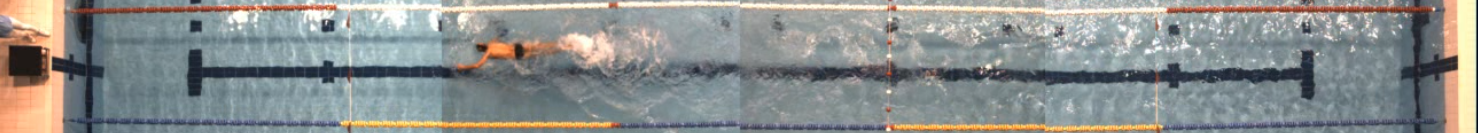
\includegraphics[width=1\textwidth,height=1\textheight,keepaspectratio]{imagenes/parte_BS/single_lane_RGB.png}   
    \caption{Calle de la piscina en espacio de color RGB.}
    \label{fig:ejemplopiscinargb}
\end{figure}

Si nos fijamos en la imagen \ref{fig:ejemplopiscinargbcanales}, donde mostramos por separado los canales RGB de un fotograma en el que sólo aparece una calle de la piscina, podremos apreciar que no existen grandes diferencias que nos permitan realizar el filtrado por el valor de uno solo de estos canales. Además, se mantienen los reflejos de los focos del pabellón sobre el agua en movimiento y el chapoteo que produce el nadador en todos los canales, lo cual podría ser considerado por el algoritmo de sustracción de fondos como movimiento, dificultando nuestra tarea.

\begin{figure}[h!]
    \centering
    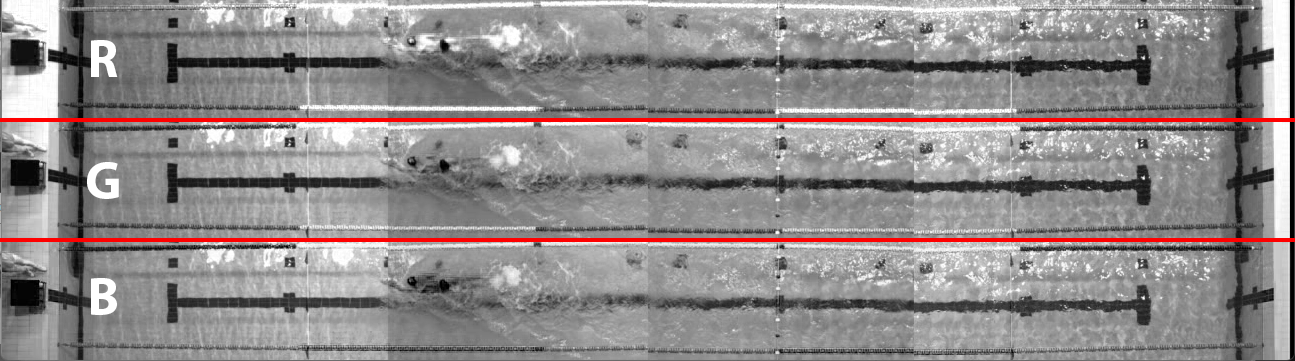
\includegraphics[width=1\textwidth,height=1\textheight,keepaspectratio]{imagenes/parte_BS/RGB_LANE.png}    
    \caption{Canales RGB por separado de una única calle de la piscina.}
    \label{fig:ejemplopiscinargbcanales}
\end{figure}

Por todos los inconvenientes expuestos, se descarta el uso el modelo de color RGB y se pasa a considerar otros modelos de color. 

En segundo lugar, consideremos el uso del espacio de color HSV. Trabajos como \cite{hsvforswimmerdetection}, \cite{pielespacioscolor} y \cite{swimmerartii} proponen el uso de este espacio de color dado que permite reducir la influencia de los cambios en la iluminación a la hora de realizar el filtrado deseado. Estos cambios, causados por reflejos en el agua, deberían quedar reflejados únicamente en las componentes de intensidad de la imagen, sin alterar la componente cromática, lo que facilita nuestra tarea de filtrado de colores. 

En la figura \ref{fig:ejemplopiscinahsvcanales} podemos apreciar el mismo fotograma que en la figura \ref{fig:ejemplopiscinargbcanales}. En esta ocasión, se muestran cada uno de los canales de la representación en el espacio de color HSV. 

\begin{figure}[h!]
    \centering
    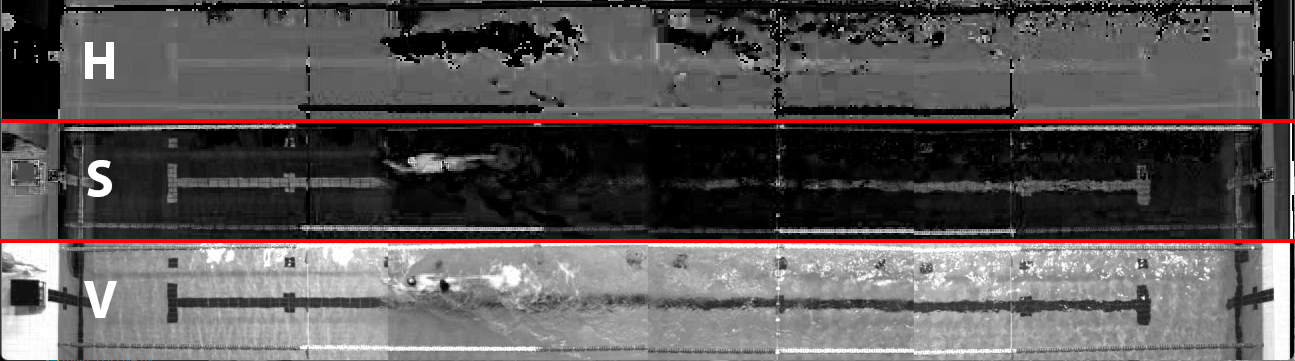
\includegraphics[width=1\textwidth,height=1\textheight,keepaspectratio]{imagenes/parte_BS/HSV_LANE.png}    
    \caption{Canales HSV de una calle de la piscina.}
    \label{fig:ejemplopiscinahsvcanales}
\end{figure}

Salta a la vista rápidamente que el canal de saturación  permite distinguir fácilmente al nadador, en colores cercanos al blanco, del resto de la escena. El agua adopta tonos oscuros, mientras que los azulejos azules del fondo de la piscina toman valores claros. Llegamos a conclusiones similares a las expuestas por los artículos anteriormente mencionados. 

Otras investigaciones, como \cite{ycbcrskini} \cite{skinvariousspaces} \cite{swimmerartii} abogan por el uso de las bandas de crominancia del espacio de color YCbCr para detectar la piel del individuo. En particular, \cite{ycbcrskini} utiliza la información de dichas bandas para calcular la cantidad de piel a la vista y decidir si una imagen es explícita o no. Nuestro objetivo final es distinto, pero compartimos similitudes con este enfoque dado que el nadador también deja gran cantidad de piel a la vista que podemos usar para diferenciarlo respecto del agua de la piscina.

En la figura \ref{fig:ejemplopiscinaycbcrcanales} podemos observar la misma situación que en figuras anteriores, pero con la diferencia de que la representación se hace por medio del espacio de color YCbCr. 

\begin{figure}[h!]
    \centering
    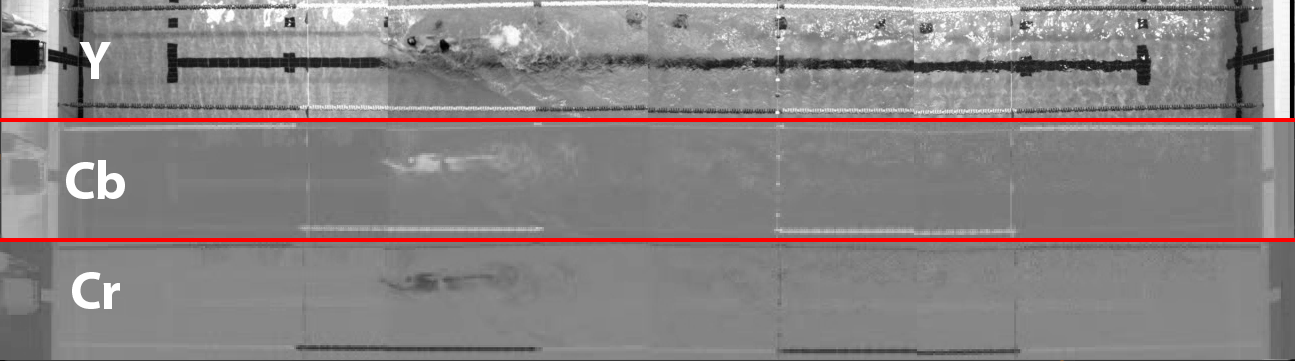
\includegraphics[width=1\textwidth,height=1\textheight,keepaspectratio]{imagenes/parte_BS/YCBCR_LANE.png}
    \caption{Canales YCbCr de una calle de la piscina.}
    \label{fig:ejemplopiscinaycbcrcanales}
\end{figure}

Si nos fijamos en las bandas de crominancia, Cb y Cr, podemos observar como el nadador es fácilmente distinguible del agua de la piscina, la cual se encuentra representada de forma bastante homogénea en un pequeño rango de colores. También podemos apreciar como no existen prácticamente reflejos en el agua proveniente de los focos del pabellón, y una menor cantidad de chapoteo que en la banda de luminancia Y. En \cite{swimmerartii} se llegan a estas mismas conclusiones, y proponen un método de detección de nadadores en función de la información que proporcionan las bandas de crominancia del espacio YCbCr.

A partir de lo mostrado en este apartado, podemos concluir que la banda de saturación del espacio HSV, y la bandas de crominancia del espacio YCbCr resultan especialmente prometedoras al permitir identificar de manera sencilla al nadador. Nuestras observaciones coinciden con la de trabajos previos como \cite{hsvforswimmerdetection} y \cite{swimmerartii}.

Evaluar experimentalmente cual de estas bandas es la más apropiada requiere de la extracción del contorno del nadador, que se discute en el apartado siguiente. Por ello, hemos pospuesto el análisis experimental a la sección \ref{sub:eleccionalgoritmo}.

\section{Sustracción de fondos} 

La sustracción de fondos es una técnica clásica del procesamiento de imágenes que permite detectar movimiento a partir de una secuencia de fotogramas capturados por una cámara estática. En su vertiente más básica, buscaremos detectar las diferencias entre el fotograma actual y el fotograma anterior, de manera que aquellos píxeles que no varíen serán considerados parte del fondo de la imagen – zonas estáticas - mientras que los píxeles cuyo valor haya sufrido cambios serán considerados parte de objetos en movimiento – zonas dinámicas. En las siguientes secciones trataremos de forma teórica los algoritmos de sustracción de fondos más populares.

\subsection{Mezcla de gaussianas}

El algoritmo de sustracción de fondos mediante “mezcla de gaussianas”, de siglas MOG, fue propuesto en el artículo \cite{origenmog}. Este método utiliza entre 3 y 5 distribuciones gaussianas de diferente media para modelar los valores en cada píxel de la imagen. Los autores de este algoritmo suponen que las diferentes distribuciones representan cada uno de los colores del fondo y primer plano de la imagen. Cada gaussiana tiene un peso asignado, el cual se va actualizando dinámicamente de forma que sea proporcional a la cantidad de tiempo que un píxel se mantiene con un determinado color. Cuando el peso de la distribución es pequeño se entiende que ese píxel cambia frecuentemente de valor, por lo que consideramos que forma parte del primer plano de la imagen.

La principal desventaja de este algoritmo es el número fijo y poco variable de distribuciones gaussianas a utilizar \cite{infomog}. Para solventar este problema se desarrolló una segunda versión del algoritmo \cite{mejoramog}, de siglas MOG2, que permite usar un número variable de distribuciones gaussianas para cada píxel en diferentes fotogramas. Al permitir una mejor representación de los colores de los píxeles, MOG2 proporciona un mejor rendimiento que la versión original del algoritmo, MOG. 

Cada implementación concreta de este algoritmo asigna un número de fotogramas previos que tener en cuenta para calcular el peso de cada distribución gaussiana durante el proceso de detección. 

\subsection{Vecinos más próximos}

En el artículo \cite{origenknn} se presenta una mejora del algoritmo basado en mezcla de gaussianas presentado en la sección anterior. Los autores utilizan ecuaciones recursivas para actualizar constantemente los parámetros de los modelos gaussianos y seleccionar el número apropiado de componentes para cada píxel. Además, se introduce el uso del algoritmo KNN para mejorar la estimación de la densidad del núcleo de las distribuciones gaussianas. 

Es esta versión mejorada del algoritmo MOG la que se conoce como algoritmo de sustracción de fondos K-NN (K vecinos más próximos) y se implementa en el paquete \textit{OpenCV}.

El algoritmo K-NN permite, a partir de un conjunto de datos etiquetados, definir un modelo de predicción con el que asignar valores de salida a datos nuevos.

Este algoritmo compara el argumento de entrada con todos los ejemplos disponibles antes de realizar una predicción. La comparación entre datos se realiza utilizando una función matemática que permita representar distancias - siendo las más comunes la distancia euclídea y la distancia de Manhattan.

Una vez se realizan las comparaciones entre datos, se tienen en consideración las K muestras más cercanas - con menor valor de distancia. Resulta de vital importancia elegir un valor del parámetro K adecuado al problema a resolver.

\subsection{Google Summer Of Code}

Vladislav Samsonov, bajo la mentoría de Maksim Shabunin, trabajó en la mejora de los algoritmos de sustracción de fondos del paquete software OpenCV durante el programa de formación \textit{Google Summer of Code} del año 2017 \cite{gsocprojectentry}. A pesar de que la propuesta inicial era la mejora del algoritmo LSBP descrito en \cite{originallbspgsoc}, su trabajo supuso además la implementación de un nuevo algoritmo para la eliminación de fondos, el cual ha recibido como nombre las siglas de dicho programa de formación, GSoC.

La implementación del algoritmo GSoC no surge ni está relacionada con ningún artículo académico, por lo que para conocer su forma de operar deberemos consultar unas breves palabras del autor \cite{gsocbytheauthor} y analizar el código fuente correspondiente a la implementación del algoritmo \cite{gsocexplainer} \cite{gsocimplementation}.

Este algoritmo utiliza descriptores de color y varias heurísticas con el objetivo de hacer el modelo más estable \cite{gsocbytheauthor}. Su principal mejora, respecto a otros algoritmos es la gestión de los píxeles parpadeantes, entendidos estos como los píxeles que cambian frecuentemente entre el primer plano - zona dinámica y el fondo de la imagen - zona estática. 

Para realizar la supresión del parpadeo necesitamos un mapa de píxeles potencialmente parpadeantes, el cual es obtenido mediante la operación lógica XOR entre la máscara del fotograma actual y el anterior. A continuación, se eligen píxeles aleatorios de entre los parpadeantes para ser sustituidos. La probabilidad con la que se realiza la sustitución depende de parámetros \textit{blinkingSupressionDecay} y \textit{blinkingSupressionMultiplier} especificados en el constructor del objeto \textit{BackgroundSubtractorGSOC} 

El valor del umbral para la eliminación del ruido se produce con la multiplicación  de los valores \textit{noiseRemovalThresholdFacBG} y \textit{noiseRemovalThresholdFacFG} en el área de la máscara. Además, los valores de la máscara se actualizan de acuerdo con el umbral obtenido.

Por último, sobre la máscara producida se realiza un procesamiento adicional, consistente en la eliminación de ruido mediante la aplicación de un filtro de desenfoque gaussiano.

\subsection{Resultados de la sustracción de fondo} \label{sub:extraccioncontornos}

Para concluir está sección, mostramos los resultados que se obtienen al aplicar el algoritmo GSoC de sustracción de fondos. Esta sección solo pretende proporcionar una idea intuitiva sobre el resultado, la comparativa cuantitativa entre los algoritmos requiere de la extracción de las bounding boxes, que se realiza posteriormente en la sección \ref{sec:Extraccion_contorno}. Nótese que tras extraer el fondo, obtenemos una imagen binaria. En aquellos píxeles en los que tenemos un valor 0 el algoritmo considera que no ha habido movimiento, mientras que en los píxeles de valor 1 se considera que se ha producido movimiento. 

A modo de ejemplo y como introducción a la sección \ref{sec:Extraccion_contorno}, en la figura \ref{fig:ejemplosinbbox} podemos observar el resultado de aplicar el algoritmo GSoC sobre la banda de crominancia roja de YCbCr de dos fotogramas. En ambos casos se puede apreciar rápidamente que el agua de la piscina queda marcada como fondo en negro, mientras que el nadador en movimiento queda marcado en blanco. 

Debemos destacar que el resultado no es perfecto; si nos fijamos en el fotograma A veremos como el bañador no se enmarca en el conjunto de píxeles blancos. Aunque pueda parecer obvio, debemos tener en cuenta que el nadador genera movimiento en el agua tras de sí conforme avanza por la piscina, en función del chapoteo que se produzca el algoritmo puede considerar este como parte del movimiento o no. En el fotograma A se puede apreciar como parte del chapoteo generado se considera movimiento, mientras que en el fotograma B la onda producida en el agua por el avance del nadador no queda enmarcada dentro del conjunto de píxeles que identifican movimiento.

\begin{figure}[h!]
    \centering
    \begin{tabular}{c}
          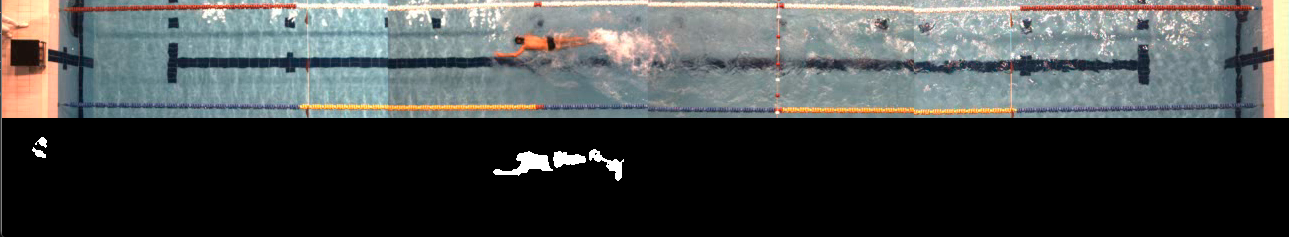
\includegraphics[width=0.9\textwidth,height=0.9\textheight,keepaspectratio]{imagenes/parte_BS/PROCESAR_SIN_BBOX_I.png} \\
          a) Fotograma A. Original y segmentación inicial. \\
          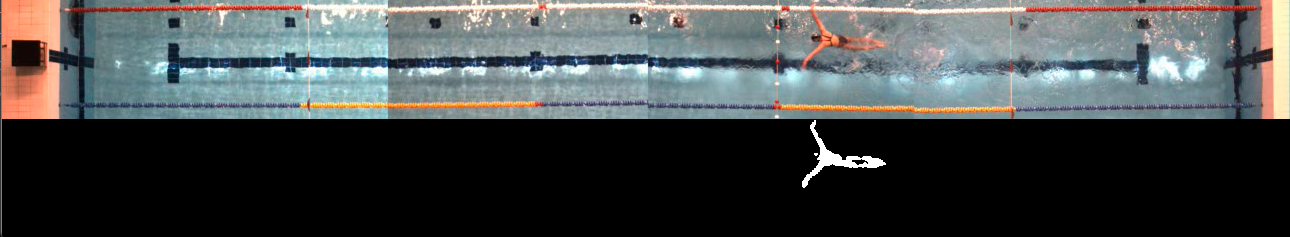
\includegraphics[width=0.9\textwidth,height=0.9\textheight,keepaspectratio]{imagenes/parte_BS/PROCESAR_SIN_BBOX_II.png} \\
          b) Fotograma B. Original y segmentación inicial. \\
     \end{tabular}
     \caption{Resultado de eliminar el fondo de la imagen utilizando GSoC sobre la banda de crominancia roja de YCbCr.}
     \label{fig:ejemplosinbbox}
\end{figure}


\section{Extracción del contorno del nadador}
\label{sec:Extraccion_contorno}
Hasta ahora hemos conseguido reconocer de manera visual al nadador, pero no hemos obtenido aún su posición en la piscina ni la zona de píxeles que le contiene. Para poder obtener una bounding box que enmarque el contorno del nadador utilizaremos la función \textit{findContours()} del paquete software OpenCV junto con un proceso de refinamiento adaptado a el modelo propuesto, y que se explica más adelante. El algoritmo implementado por dicho software se basa en \cite{contornosalgor}, y trabaja sobre imágenes binarias buscando unir aquellos píxeles con valor no nulo que estén 4-conectados u 8-conectados. Además, tiene en cuenta cuales son los píxeles externos y la jerarquía entre conexiones para poder ofrecer tolerancia a pequeños huecos que puedan producirse en el interior del objeto a delimitar.

Para nuestros experimentos, hemos utilizado las siguientes banderas: \\\textit{RETR\_EXTERNAL} y \textit{CHAIN\_APPROX\_SIMPLE}. De esta manera, sólo obtenemos las bounding box exteriores, representadas cada una de ellas por una tupla de la forma [coordenada X, coordenada Y, ancho, alto]. Este enfoque nos permite ahorrar memoria de forma significativa, ya que solo deberemos almacenar 4 valores enteros por bounding box, en lugar de las coordenadas X e Y de cada punto que conforme cada contorno, las cuales no necesitaremos.

En la figura \ref{fig:muchoscontornos} se muestran varios fotogramas, sobre los que se han dibujado rectángulos correspondientes a los contornos detectados.

\begin{figure}[h!]
    \centering
    \begin{tabular}{c}
          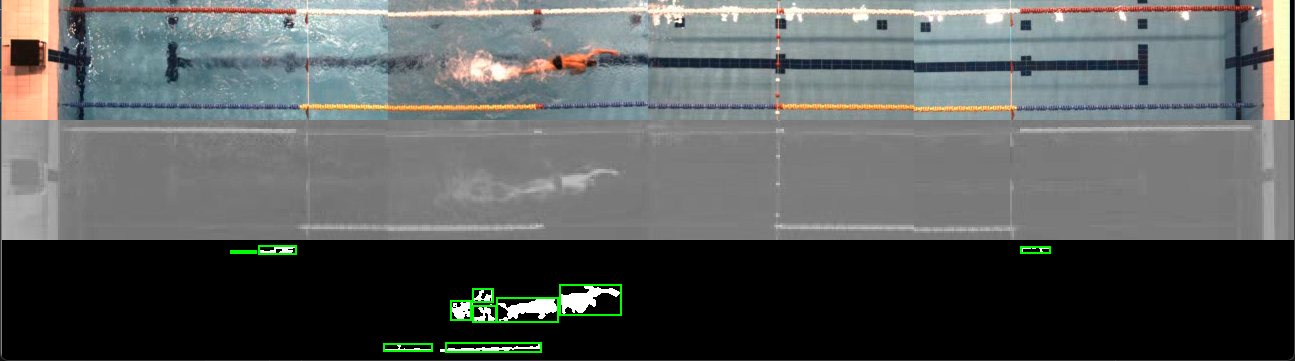
\includegraphics[width=0.9\textwidth,height=0.9\textheight,keepaspectratio]{imagenes/parte_BS/MUCHOS_CONTORNOS_I.png} \\
          a) Fotograma A y bounding boxes detectadas. \\
          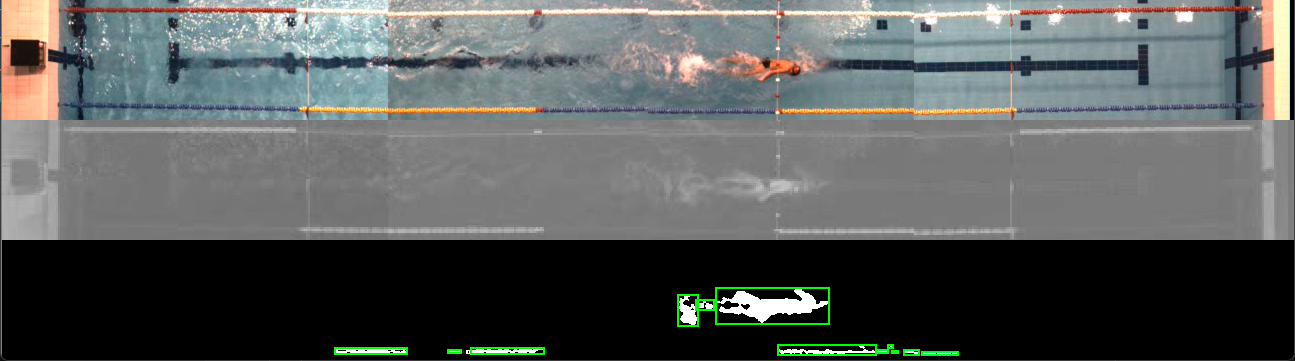
\includegraphics[width=0.9\textwidth,height=0.9\textheight,keepaspectratio]{imagenes/parte_BS/MUCHOS_CONTORNOS_II.png} \\
          b) Fotograma B y bounding boxes detectadas.\\
          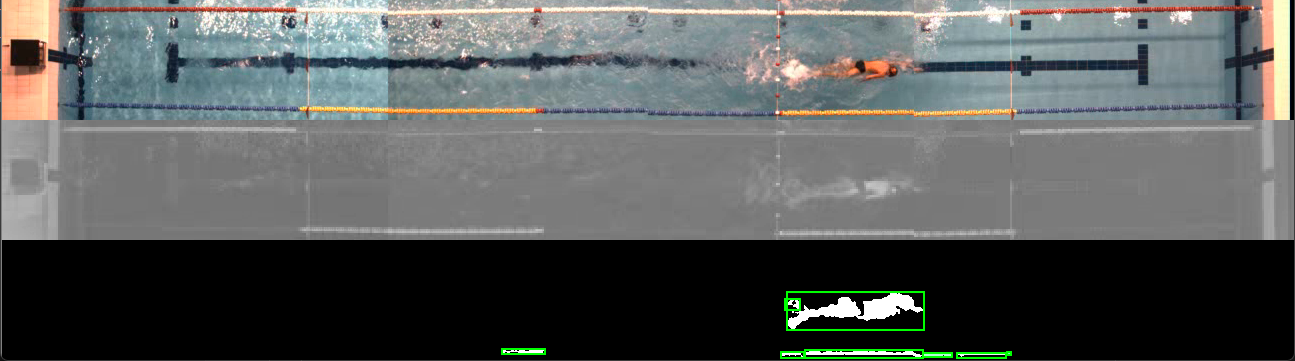
\includegraphics[width=0.9\textwidth,height=0.9\textheight,keepaspectratio]{imagenes/parte_BS/MUCHOS_CONTORNOS_III.png} \\
          c) Fotograma C y bounding boxes detectadas.\\
     \end{tabular}
     \caption{Bounding boxes detectadas sin proceso de filtrado.}
     \label{fig:muchoscontornos}
\end{figure}

Analicemos los distintos fotogramas y sus peculiaridades uno por uno. 
\begin{itemize}
    \item En el fotograma A podemos observar como se detectan múltiples bounding boxes. Particularmente, tenemos parte de las corcheras, el nadador dividido en dos - dado que el bañador no detectado genera una discontinuidad en el borde - y varios cajas correspondientes al chapoteo generado por las patadas del nadador.
    \item En el fotograma B seguimos manteniendo la detección de algunas corcheras. Sin embargo, en esta ocasión el contorno del nadador sí que es detectado como una sola entidad, bajo un único rectángulo.
    \item En el fotograma C el movimiento del agua tras el nadador es tan considerable que el algoritmo recoge al nadador y parte de dicho agua  bajo una única bounding box. Inicialmente se barajó la posibilidad de utilizar morfología matemática para intentar eliminar el efecto del chapoteo en el agua. Sin embargo, su aplicación con diversas formas y tamaños no produjo resultados satisfactorios y se descartó su uso. Ciertamente se conseguía reducir la cantidad de chapoteo reconocida como parte del nadador, pero también se desvirtuaba considerablemente el contorno del nadador, de forma que no resultaba útil para el cálculo de la frecuencia de nado.
\end{itemize}

Tras delimitar los posibles objetos, tendremos en cuenta las características de cada tipo de fotograma para diseñar un proceso de refinamiento que nos permita obtener como resultado final una única bounding box que enmarque el contorno del nadador. Los pasos que se seguirán en dicho proceso son los siguientes:

\begin{enumerate}
    \item En primer lugar discriminaremos las bounding boxes obtenidas en función de su posición en el eje X. Sólo nos interesaran aquellas que se encuentren dentro del agua de la piscina. Esta medida puede parecer innecesaria, ya que la parte del fotograma que no abarca la piscina es muy pequeña, pero no lo es. Hay ocasiones en los que el entrenador se acerca al borde del trampolín para dar instrucciones al nadador, o hay personas deambulando por esa zona. Estos sujetos no son de nuestro interés, por lo que debemos descartarlos. 
    \item A continuación, buscaremos obviar las corcheras que separan las calles de las piscinas. Dado que la posición de las corcheras no varía significativamente, ya que siempre están en los mismos lugares de la piscina y el nado de otros nadadores de calles contiguas apenas las mueven, podemos discriminarlas en función de su posición. Así pues, descartaremos los objetos cuyas coordenadas Y (superior izquierda del rectángulo) se encuentre en el 10\% superior o 10\% inferior de la calle. Además, dado que las corcheras tienen un tamaño homologado, también las discriminaremos por su altura, la cual es bastante inferior al ancho de un humano. Colateralmente, estas restricciones nos permite obviar personas que deambulen por el borde de la primera y última calle.
    \item Una vez hemos seleccionado las bounding boxes pertenecientes a la región de interés de la calle, realizaremos un filtrado en función del área. En los fotogramas de la figura \ref{fig:muchoscontornos} se puede observar que las bounding boxes que contienen al nadador son las de mayor área. Dado que el nadador puede representarse mediante dos bounding boxes, al separarse tronco de piernas, o en una única bounding box, debemos buscar valores experimentales que nos indiquen un área mínima y máxima para la cual consideramos que la bounding box puede pertenecer a un nadador. De detectarse más de dos objetos, nos quedaremos sólo con las dos bounding boxes de mayor área cuyo valor se encuentre en el rango anteriormente calculado. Esta medida nos permite obviar bounding boxes que contengan zonas de agua en movimiento debido a las patadas del nadador.
    
    \item Por último, distinguiremos en función de si tenemos una o dos bounding boxes. En caso de tener una única bounding box consideraremos que este es el nadador, mientras que en el caso de que tengamos dos bounding boxes consideraremos que podrían contener tronco y piernas del nadador e intentaremos unirlas. Tendremos en cuenta tres factores a la hora de decidir si unir las cajas o no. 
        \begin{itemize}
            \item La separación vertical entre las bounding box. La esquina superior izquierda de las bounding box que contienen tronco superior y las piernas del nadador deberían tener aproximadamente la misma posición en el eje Y, teniendo en cuenta un margen de error dado que el brazo puede estar extendido si se está realizando una brazada.
            \item La separación en el eje X entre ambas cajas. El hecho de que el nadador se detecte en dos bounding boxes separadas suele atribuirse a que el bañador no es detectado por el algoritmo de sustracción de fondos. Si la separación entre las cajas es significativamente mayor que el tamaño de un bañador consideraremos que no se deben unir.
            \item La longitud posible de la bounding box resultante de la unión. Resulta lógico descartar la unión de las bounding boxes cuando esta pueda generar resultados poco realistas. Por ejemplo, es altamente improbable que el nadador a seguir mida más de 2.3 metros. La excesiva longitud de la bounding box resultante suele producirse debido a una cantidad significativa de chapoteo detectada como parte de las piernas del nadador. Este parámetro es difícil de ajustar dada la gran variación en estatura que puede haber entre nadadores, así como la variación en el tamaño del chapoteo generado por sus patadas.
        \end{itemize}
    La unión de las bounding box sólo se realizará si los tres valores anteriormente mencionados se encuentran dentro de unos determinados rangos, calculados experimentalmente a partir de los datos que hemos podido extraer y analizar de las bounding box generadas en torno a los nadadores en varios vídeos. 
\end{enumerate}

Una vez tenemos una única bounding box, que hemos considerado que enmarca el contorno del nadador, guardaremos su posición en el eje X y su anchura. Estos datos los analizaremos en el capítulo \ref{cap:capitulo5} para poder calcular la frecuencia media de nado. Con la extracción de la bounding box ya estamos en posición de evaluar cuantitativamente las distintas combinaciones de espacio de color y algoritmo de sustracción de fondo. Los resultados experimentales se muestran a continuación en la sección \ref{sub:eleccionalgoritmo}.

\section{Evaluación experimental} \label{sub:eleccionalgoritmo}

En las secciones anteriores hemos comentado los espacios de color, algoritmos de sustracción de fondos más populares y cómo extraemos el contorno del nadador en forma de bounding box. En esta sección nos centraremos en analizar el rendimiento de nuestro método para las distintas combinaciones posibles que pueden tener lugar a partir de los espacios de color descritos en \ref{sub:elegirespaciocolor} y los algoritmos de sustracción de fondos explicados. Elegiremos aquella combinación que mejores resultados prácticos nos proporcione.

Para evaluar los resultados, usaremos los vídeos proporcionados por investigadores de la Facultad de Ciencias del Deporte de la Universidad de Granada. Sin embargo, carecemos de etiquetas sobre la posición exacta del nadador en cada fotograma. Con el objetivo de disponer de información que nos permita evaluar cuantitativamente los resultados, hemos seleccionado aleatoriamente 45 fotogramas de entre los vídeos que tenemos a nuestra disposición. Los fotogramas muestran una única calle de la piscina y se ha etiquetado manualmente el contorno del nadador mediante una bounding box.

Para realizar la comparativa emplearemos dos métricas, el índice de Jaccard y el coeficiente de Sorensen-Dice. Estos nos permitirán determinar cómo de buena es la bounding box que el algoritmo nos devuelve frente a una bounding box determinada manualmente por un humano.

\begin{itemize}
    \item El índice de Jaccard, también conocido como ``intersección sobre la unión`` (IoU), es una de las métricas más utilizadas en segmentación de imágenes debido a su sencillez y efectividad. Nos permite medir el grado de superposición de dos bounding boxes, cuanto más se solapen, mayor será el valor del índice. Su expresión matemática es la siguiente: 
    \begin{equation}
        IoU= \frac{Area\ de\ interseccion}{Area\ de\ union} = \frac{A \cap B}{A \cup B}=\frac{A\cap B}{|A|+|B|-(A \cap B)}
    \end{equation}
    \item El coeficiente de Sorensen-Dice, también conocido como F1-Score, es otra de las métricas más utilizadas, y nos permite combinar la precisión - cuantas predicciones positivas son realmente positivas - y el recall - cuántas predicciones positivas están realmente bien clasificadas - en una única métrica. Este índice trata mejor a aquellos algoritmos que consigan realizar predicciones correctas, verdaderos positivos. Su expresión matemática es la siguiente: 
    \begin{equation}
        Dice = \frac{2 \times Area\ de\ interseccion}{Suma\ de\ cardinalidades} = \frac{2 \times (A \cap B)}{|A| + |B|}
    \end{equation}
\end{itemize}

Ambos índices están positivamente correlados, es decir, si uno de ellos dice que el método A es mejor que el método B, el otro dirá lo mismo. Además, ambos índices varían en el rango [0,1]; siendo 0 una predicción totalmente incorrecta y 1 la similitud total entre las bounding boxes. 

En la figura \ref{fig:iouvisualimgs} se muestran 6 fotogramas en los que se comparan las predicciones realizadas por el algoritmo, representadas en rojo, con la segmentación realizada manualmente por un humano, en verde. En dichas imágenes se recogen situaciones a las que suele enfrentarse el algoritmo. En particular:
\begin{itemize}
    \item En los fotogramas A y B no se cumple el criterio para unir tren superior e inferior del nadador, por lo que sólo se considera la región de mayor área. Por lo general, el tren superior ocupa un mayor área que el tren inferior, especialmente si los brazos se encuentran estirados o se está realizando una brazada.
    \item En los fotogramas C y D sí que se detecta al nadador completo, pero también se considera como parte del nadador una buena parte del chapoteo que genera su avance por el agua. Como veremos posteriormente, esto disminuirá la calidad de la segmentación realizada.
    \item En los fotogramas E y F se consigue detectar al nadador sin incluir casi chapoteo alguno. Este es el caso que desearíamos que siempre se produjera.
\end{itemize}  

Con el objetivo de ilustrar el comportamiento de las métricas ante distintas situaciones, en la tabla \ref{tab:iouvisualtab} se recogen los valores de los índices de Jaccard y Sorensen-Dice para cada fotograma de la figura \ref{fig:iouvisualimgs}. Si se comparan los valores numéricos con los resultados visuales, se pueden extraer importantes conclusiones:
\begin{itemize}
    \item Las predicciones en las que sólo se detecte correctamente a medio nadador tienen valores de los coeficientes de Jaccard y Sorensen-Dice bajos. Sus valores suelen oscilar en el rango [0.2; 0.45]. 
    \item En el caso de detectar como parte del nadador chapoteo del agua, el valor de los índices se mueve en un rango relativamente amplio. En los casos extremo en los que se detecta todo el chapoteo como parte del nadador, como en el fotograma C, el índice de Jaccard tiene un valor en el rango [0.3; 0.37] aproximadamente. Si se detecta poco chapoteo el valor del índice de Jaccard suele encontrarse en el rango [0.55; 0.65]. Podríamos considerar como buenas predicciones, por tanto, aquellas que superen un valor IoU de 0.55.
    \item En el caso de detecciones muy buenas, como en el fotograma E, o prácticamente perfectas, como en fotograma F, el índice de Jaccard tiene un valor en el rango [0.8; 0.9], mientras que el índice de Sorensen-Dice se mueve en el rango [0.88; 0.95].
\end{itemize}
 
\begin{figure}[h!]
    \centering
    \begin{tabular}{cc}
          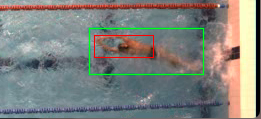
\includegraphics[width=0.43\textwidth,height=0.43\textheight,keepaspectratio]{imagenes/parte_BS/iou_visual/mala_1099.png} &
          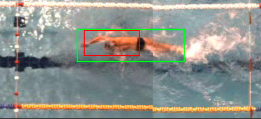
\includegraphics[width=0.43\textwidth,height=0.43\textheight,keepaspectratio]{imagenes/parte_BS/iou_visual/medio_cuerpo_1259.png}
          \\ Fotograma A   & Fotograma B \\
          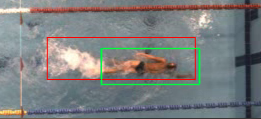
\includegraphics[width=0.43\textwidth,height=0.43\textheight,keepaspectratio]{imagenes/parte_BS/iou_visual/muchisima_agua_1014.png} &
          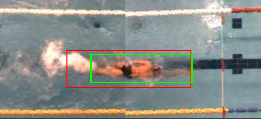
\includegraphics[width=0.43\textwidth,height=0.43\textheight,keepaspectratio]{imagenes/parte_BS/iou_visual/mucha_agua_897.png}
          \\ Fotograma C & Fotograma D \\
          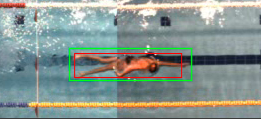
\includegraphics[width=0.43\textwidth,height=0.43\textheight,keepaspectratio]{imagenes/parte_BS/iou_visual/excelente_611.png} &
          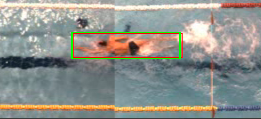
\includegraphics[width=0.43\textwidth,height=0.43\textheight,keepaspectratio]{imagenes/parte_BS/iou_visual/excelentisimo_1241.png}
          \\Fotograma E & Fotograma F
     \end{tabular}
     \caption{Predicción automática (en rojo) frente a segmentación manual (en verde) para diferentes fotogramas}
     \label{fig:iouvisualimgs}
\end{figure}

\begin{table}[h!]
    \centering
    \begin{tabular}{| c | c | c | } \hline
        Fotograma & IoU & Sorensen-Dice \\ \hline
        A & 0.23627 & 0.38223  \\
        B & 0.40158 & 0.57304 \\   
        C & 0.35484 & 0.52381 \\ 
        D & 0.60322 & 0.75251 \\ 
        E & 0.82480 & 0.90399 \\ 
        F & 0.87036 & 0.93069 \\ \hline
    \end{tabular}
    \caption{Métricas para predicciones frente a segmentación manual}
    \label{tab:iouvisualtab}
\end{table}


\begin{table}
    \centering
    \begin{tabular}{| c | c | c | c | c|}\hline
        %\multirow{number rows}{width}{text} &  \\
        Banda & Algoritmo & IoU & Dice & T.ejecución (ms) \\ \hline
        \multirow{3}{*}{S de HSV} & KNN  & 0.47256 & 0.56733 & 5.530 \\
        &MOG2 & 0.49366 & 0.59887 & 5.457 \\
        &GSoC & 0.48128 & 0.57142 & 11.778 \\ \hline
        \multirow{3}{*}{Cb de YCbCr} & KNN  & 0.14175 & 0.22651 & \textbf{3.918} \\
        &MOG2 & 0.39959 & 0.53033 & 4.099 \\
        &GSoC & 0.47209 & 0.61864 & 10.939 \\ \hline
        \multirow{3}{*}{Cr de YCbCr} & KNN  & 0.39881 & 0.55140 & 4.423 \\
        &MOG2 & 0.56134 & 0.68497 & 4.413 \\
        &GSoC & \textbf{0.64126} & \textbf{0.76864} & 11.051 \\ \hline
    \end{tabular}
    \caption{Comparativa de rendimiento}
    \label{tab:rendimientofondoscap3}
\end{table}

En las tablas de la figura \ref{tab:rendimientofondoscap3} se muestran los resultados experimentales obtenidos en media para todo el dataset de evaluación. Adicionalmente, se proporciona el tiempo medio en milisegundos que ha demorado la ejecución para cada fotograma de un vídeo de 2025 fotogramas de longitud. 

Analicemos los resultados de las tablas anteriores para elegir una combinación de espacio de color y algoritmo de sustracción de fondos a utilizar.
\begin{itemize}
    \item Para el caso del canal de saturación de HSV podemos concluir que la influencia del algoritmo de sustracción es muy pequeña. Los algoritmos K-NN y GSoC nos devuelven valores prácticamente iguales para las métricas consideradas, siendo el algoritmo MOG2 el que ofrece resultados ligeramente mejores, con un valor IoU 0.015 mayor. Si tuviéramos que trabajar en esta banda la elección más recomendable, bajo nuestra opinión, sería el algoritmo MOG2. Esto es debido a que la diferencia de rendimiento respecto de los demás algoritmos no es demasiado significativa, y el tiempo de ejecución es similar al de KNN. Las métricas nos indican que el uso de esta banda nos devolvería predicciones que podríamos considerar acertadas, pero no excelentes.
    \item En la banda de crominancia azul de YCbCr sí que notamos diferencia al utilizar distintos algoritmos. El algoritmo K-NN ofrece resultados pésimos, al proporcionar un valor del índice de Jaccard significativamente menor a 0.3. MOG2 y GSoC ofrecen predicciones algo más certeras, siendo GSoC el que mejor se comporta. En virtud de los valores experimentales podemos concluir que el uso de esta banda no ofrece mejora alguna respecto de la banda de saturación de HSV, por lo que la descartamos como posible elección.
    \item Los mejores resultados medios los obtenemos haciendo uso del canal de crominancia roja de YCbCr. Para este canal, el algoritmo con menor rendimiento (K-NN) ya proporciona resultados que podríamos considerar aceptables, al tener un valor del índice de Jaccard de 0.4. Sin embargo, podemos observar que el algoritmo GSoC obtiene un resultado medio bastante mejor, con un valor de los índices IoU y Sorensen-Dice de 0.64 y 0.769, respectivamente. Si comparamos estos valores con los mostrados en la tabla \ref{tab:iouvisualtab}, correspondientes a los fotogramas de la figura \ref{fig:iouvisualimgs}, podemos concluir que las predicciones son ciertamente buenas, y como veremos posteriormente en el capítulo \ref{cap:capitulo5}, suficientes para realizar la estimación de las brazadas por minuto del nadador. A pesar de que GSoC requiere algo más del doble de tiempo de cómputo que otros algoritmos, podríamos satisfacer condiciones de tiempo real si fuese necesario. Si tenemos en cuenta que los vídeos proporcionados por los investigadores tienen una tasa de 41.66 fotogramas por segundo necesitaríamos procesar y mostrar un fotograma cada 24 milisegundos para mantener la fluidez del vídeo. Dado que ambos métodos ofrecen un tiempo de ejecución considerablemente menor a los mencionados 24 milisegundos podemos elegir cualquiera de ellos. Por tanto, elegiremos la banda de crominancia roja de YCbCr y el algoritmo GSoC para realizar la detección del nadador al ser los que mejores resultados proporcionan. 
\end{itemize}

Por último, se debe tener en cuenta que se requieren unos doscientos fotogramas, aproximadamente, para entrenar el modelo del sustractor de fondos GSoC, de manera que se produzca la eliminación del fondo con el nivel de rendimiento esperado. En el dominio de nuestro problema, 200 fotogramas equivalen a unos 4.5 segundos. Si tenemos en cuenta el tiempo que toma iniciar la grabación y avisar al entrenador de que puede indicar la salida al nadador, la preparación del propio nadador, y el inicio de la prueba, el entrenamiento del modelo se realiza a tiempo, por lo que no encontramos problemas prácticos. Cuando el nadador se lanza a la piscina el modelo ya es capaz de categorizar la inmensa mayoría del agua como elemento estático y realizar una correcta eliminación del fondo.

Tras analizar el método que utilizaremos para detectar al nadador a lo largo de la piscina siguiendo técnicas clásicas del procesamiento de imágenes, en el siguiente capítulo se comentará un método para realizar la detección haciendo uso de técnicas de aprendizaje profundo y redes neuronales.